\documentclass[11pt]{article}
\usepackage[textwidth=18.0cm, textheight=23.0cm, top=2.0cm]{geometry}
\usepackage{pst-all}
\usepackage{amssymb}
\usepackage{tikz}
\usepackage{underscore}\begin{document}
\pagestyle{empty}


ClassName: \underline{\textbf{Class_10.2bp-29}}
\par
BinSize: \underline{\textbf{100 × 100}}
\par
ReduceSize: \underline{\textbf{100 × 100}}
\par
TypeNum: \underline{\textbf{59}}
\par
Num: \underline{\textbf{60}}
\par
OutS: \underline{\textbf{80000}}
\par
InS: \underline{\textbf{73074}}
\par
Rate: \underline{\textbf{0.913}}
\par
UB: \underline{\textbf{8}}
\par
LB0: \underline{\textbf{8}}
\par
LB: \underline{\textbf{8}}
\par
LBWithCut: \underline{\textbf{8}}
\par
NodeCut: \underline{\textbf{0}}
\par
ExtendedNodeCnt: \underline{\textbf{1}}
\par
GenNodeCnt: \underline{\textbf{1}}
\par
PrimalNode: \underline{\textbf{0}}
\par
ColumnCount: \underline{\textbf{8}}
\par
TotalCutCount: \underline{\textbf{0}}
\par
RootCutCount: \underline{\textbf{0}}
\par
LPSolverCnt: \underline{\textbf{1}}
\par
PricingSolverCnt: \underline{\textbf{0}}
\par
BranchAndBoundNum: \underline{\textbf{1}}
\par
isOpt: \underline{\textbf{true}}
\par
TimeOnInitSolution: \underline{\textbf{600.000 s}}
\par
TimeOnPrimal: \underline{\textbf{0.000 s}}
\par
TimeOnPricing: \underline{\textbf{0.000 s}}
\par
TimeOnRmp: \underline{\textbf{0.063 s}}
\par
TotalTime: \underline{\textbf{600.313 s}}
\par
\newpage


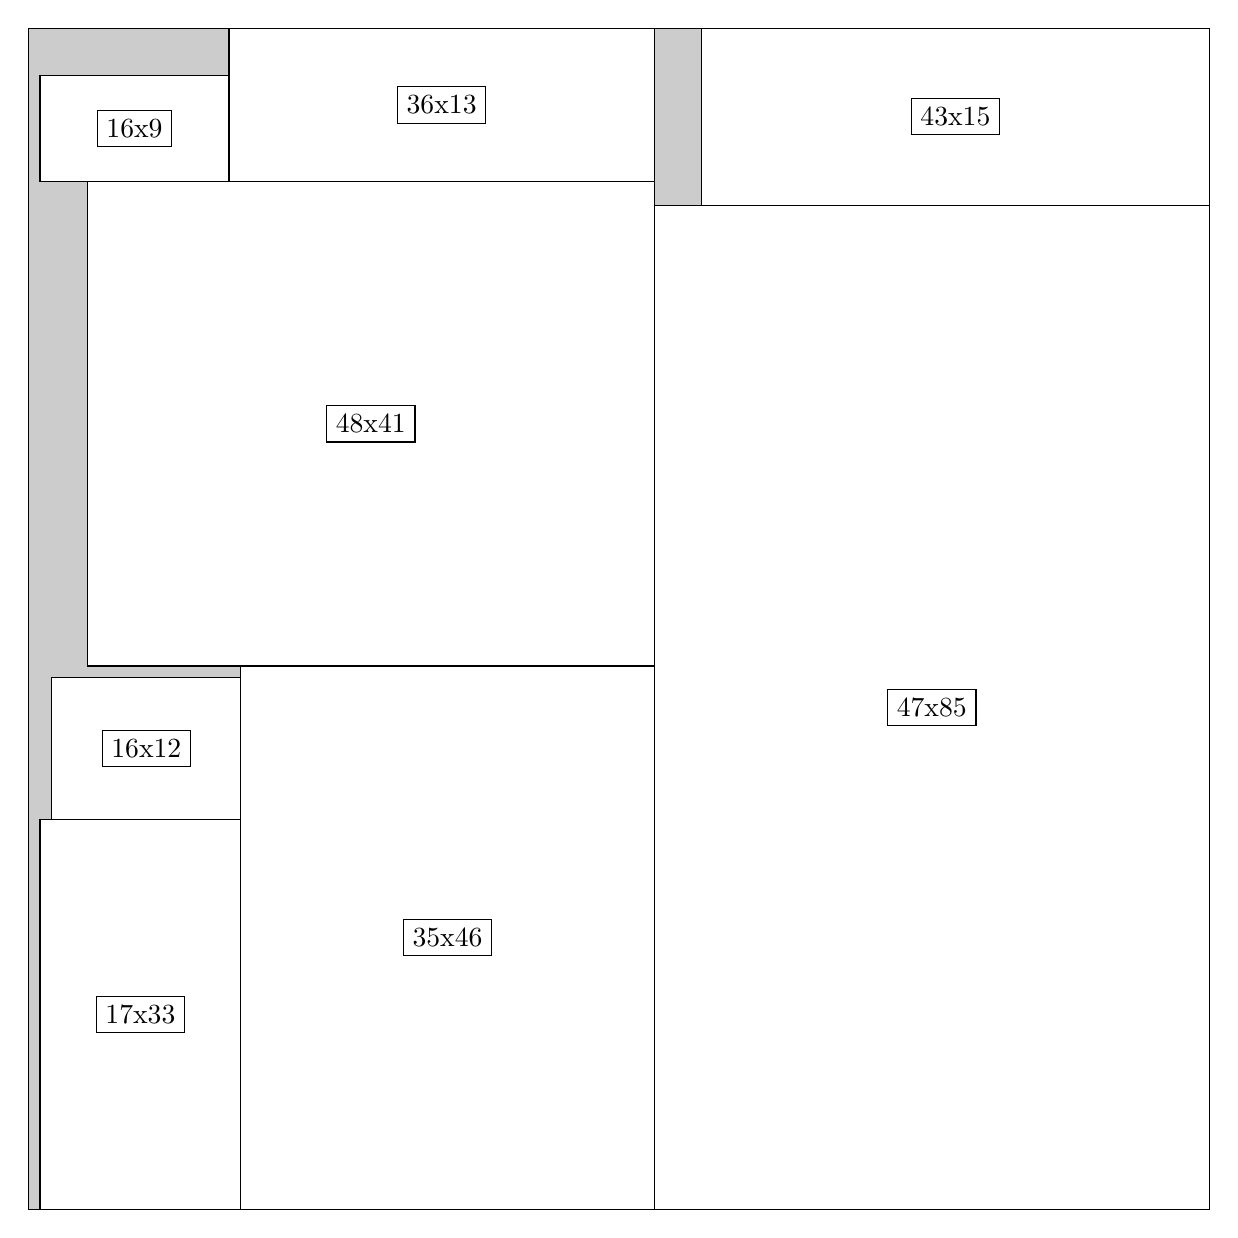
\begin{tikzpicture}[shorten >=1pt,scale=1.0,every node/.style={scale=1.0},->]
\tikzstyle{vertex}=[circle,fill=black!25,minimum size=14pt,inner sep=0pt]
\filldraw[fill=gray!40!white, draw=black] (0,0) rectangle (15.0,15.0);
\foreach \name/\x/\y/\w/\h in {47x85/7.949999999999999/0.0/7.05/12.75,43x15/8.549999999999999/12.75/6.45/2.25,35x46/2.6999999999999997/0.0/5.25/6.8999999999999995,17x33/0.15/0.0/2.55/4.95,16x12/0.3/4.95/2.4/1.7999999999999998,48x41/0.75/6.8999999999999995/7.199999999999999/6.1499999999999995,36x13/2.55/13.049999999999999/5.3999999999999995/1.95,16x9/0.15/13.049999999999999/2.4/1.3499999999999999}
\filldraw[fill=white!40!white, draw=black] (\x,\y) rectangle node[draw] (\name) {\name} ++(\w,\h);
\end{tikzpicture}


w =47 , h =85 , x =53 , y =0 , v =3995
\par
w =43 , h =15 , x =57 , y =85 , v =645
\par
w =35 , h =46 , x =18 , y =0 , v =1610
\par
w =17 , h =33 , x =1 , y =0 , v =561
\par
w =16 , h =12 , x =2 , y =33 , v =192
\par
w =48 , h =41 , x =5 , y =46 , v =1968
\par
w =36 , h =13 , x =17 , y =87 , v =468
\par
w =16 , h =9 , x =1 , y =87 , v =144
\par
\newpage


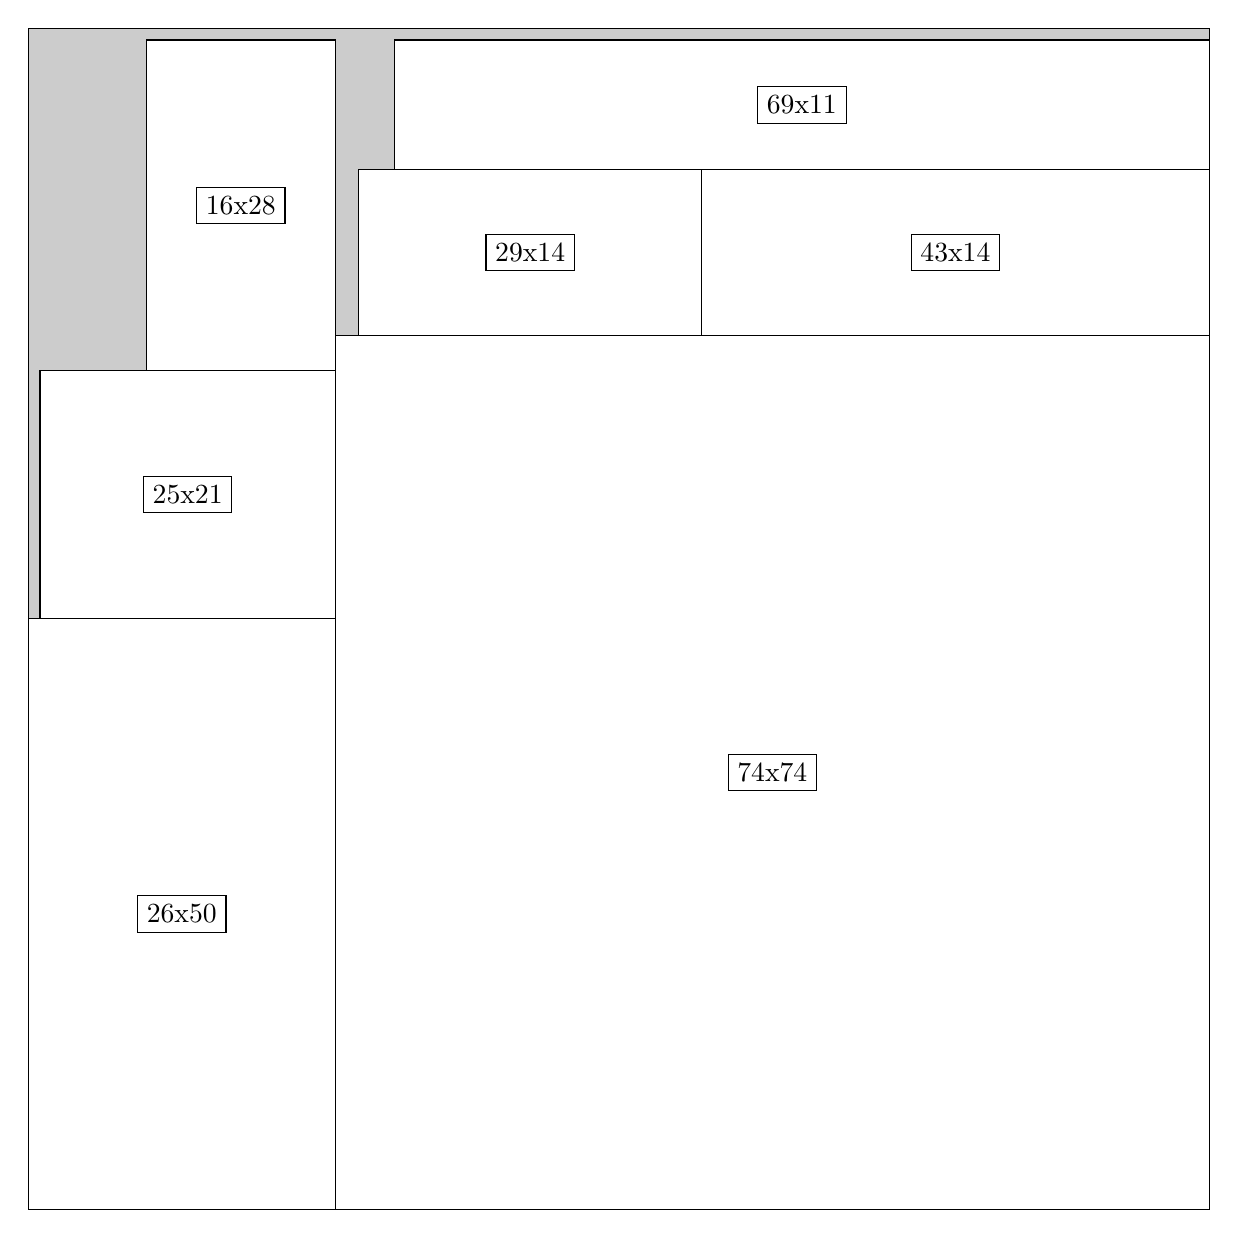
\begin{tikzpicture}[shorten >=1pt,scale=1.0,every node/.style={scale=1.0},->]
\tikzstyle{vertex}=[circle,fill=black!25,minimum size=14pt,inner sep=0pt]
\filldraw[fill=gray!40!white, draw=black] (0,0) rectangle (15.0,15.0);
\foreach \name/\x/\y/\w/\h in {74x74/3.9/0.0/11.1/11.1,43x14/8.549999999999999/11.1/6.45/2.1,29x14/4.2/11.1/4.35/2.1,69x11/4.6499999999999995/13.2/10.35/1.65,26x50/0.0/0.0/3.9/7.5,25x21/0.15/7.5/3.75/3.15,16x28/1.5/10.65/2.4/4.2}
\filldraw[fill=white!40!white, draw=black] (\x,\y) rectangle node[draw] (\name) {\name} ++(\w,\h);
\end{tikzpicture}


w =74 , h =74 , x =26 , y =0 , v =5476
\par
w =43 , h =14 , x =57 , y =74 , v =602
\par
w =29 , h =14 , x =28 , y =74 , v =406
\par
w =69 , h =11 , x =31 , y =88 , v =759
\par
w =26 , h =50 , x =0 , y =0 , v =1300
\par
w =25 , h =21 , x =1 , y =50 , v =525
\par
w =16 , h =28 , x =10 , y =71 , v =448
\par
\newpage


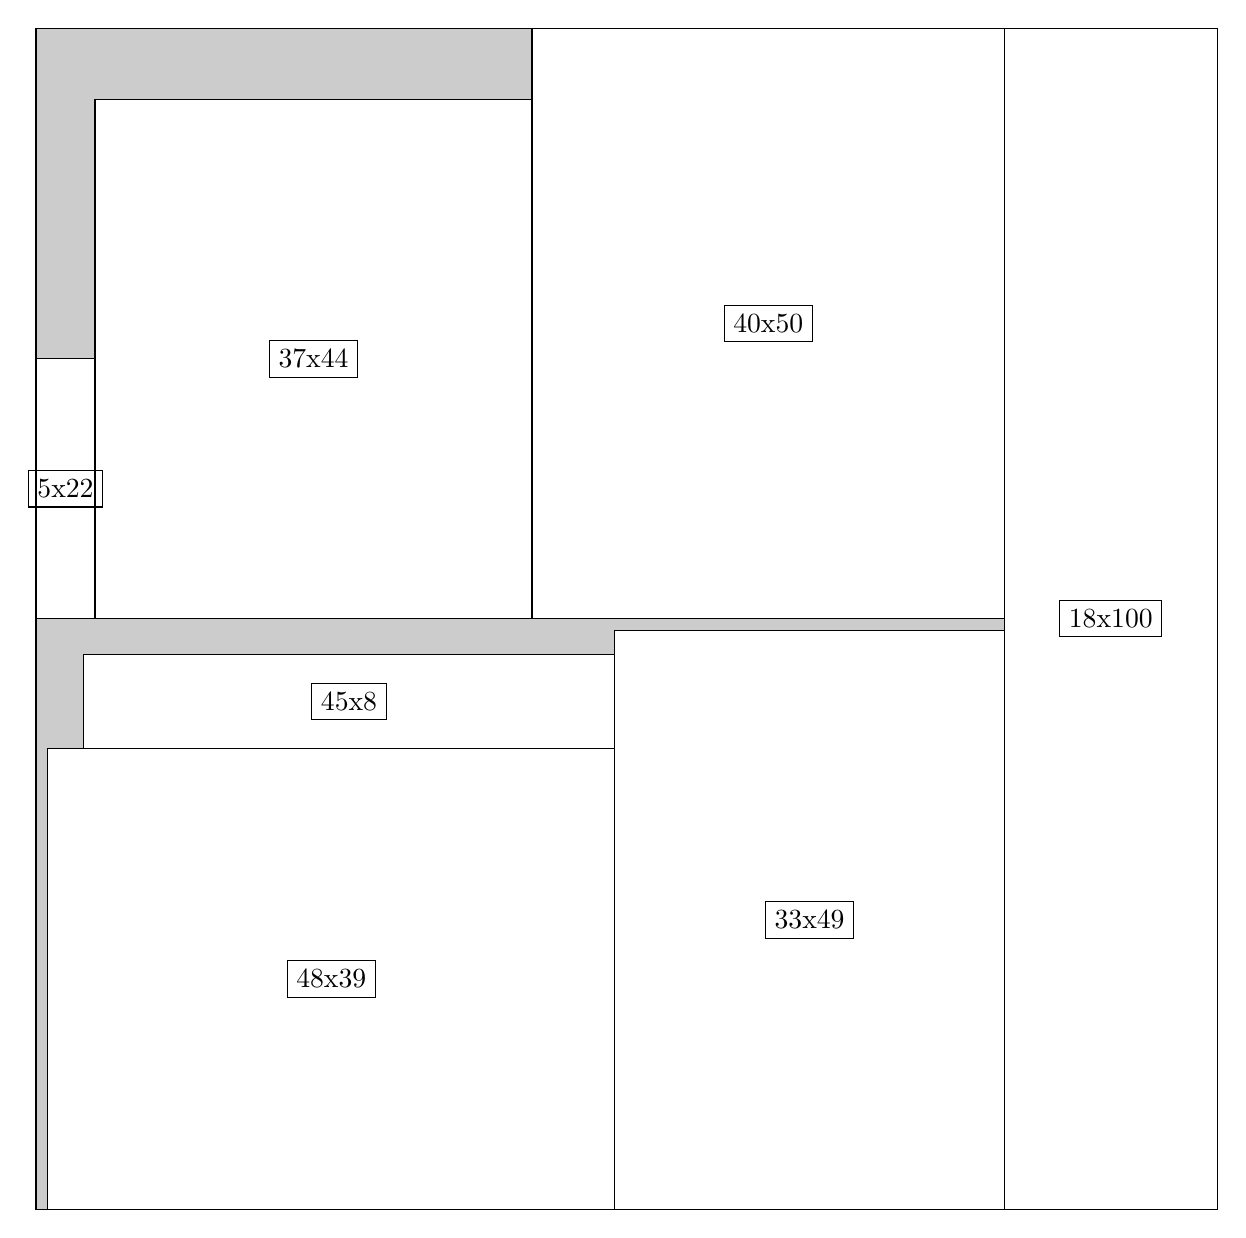
\begin{tikzpicture}[shorten >=1pt,scale=1.0,every node/.style={scale=1.0},->]
\tikzstyle{vertex}=[circle,fill=black!25,minimum size=14pt,inner sep=0pt]
\filldraw[fill=gray!40!white, draw=black] (0,0) rectangle (15.0,15.0);
\foreach \name/\x/\y/\w/\h in {18x100/12.299999999999999/0.0/2.6999999999999997/15.0,33x49/7.35/0.0/4.95/7.35,48x39/0.15/0.0/7.199999999999999/5.85,45x8/0.6/5.85/6.75/1.2,40x50/6.3/7.5/6.0/7.5,37x44/0.75/7.5/5.55/6.6,5x22/0.0/7.5/0.75/3.3}
\filldraw[fill=white!40!white, draw=black] (\x,\y) rectangle node[draw] (\name) {\name} ++(\w,\h);
\end{tikzpicture}


w =18 , h =100 , x =82 , y =0 , v =1800
\par
w =33 , h =49 , x =49 , y =0 , v =1617
\par
w =48 , h =39 , x =1 , y =0 , v =1872
\par
w =45 , h =8 , x =4 , y =39 , v =360
\par
w =40 , h =50 , x =42 , y =50 , v =2000
\par
w =37 , h =44 , x =5 , y =50 , v =1628
\par
w =5 , h =22 , x =0 , y =50 , v =110
\par
\newpage


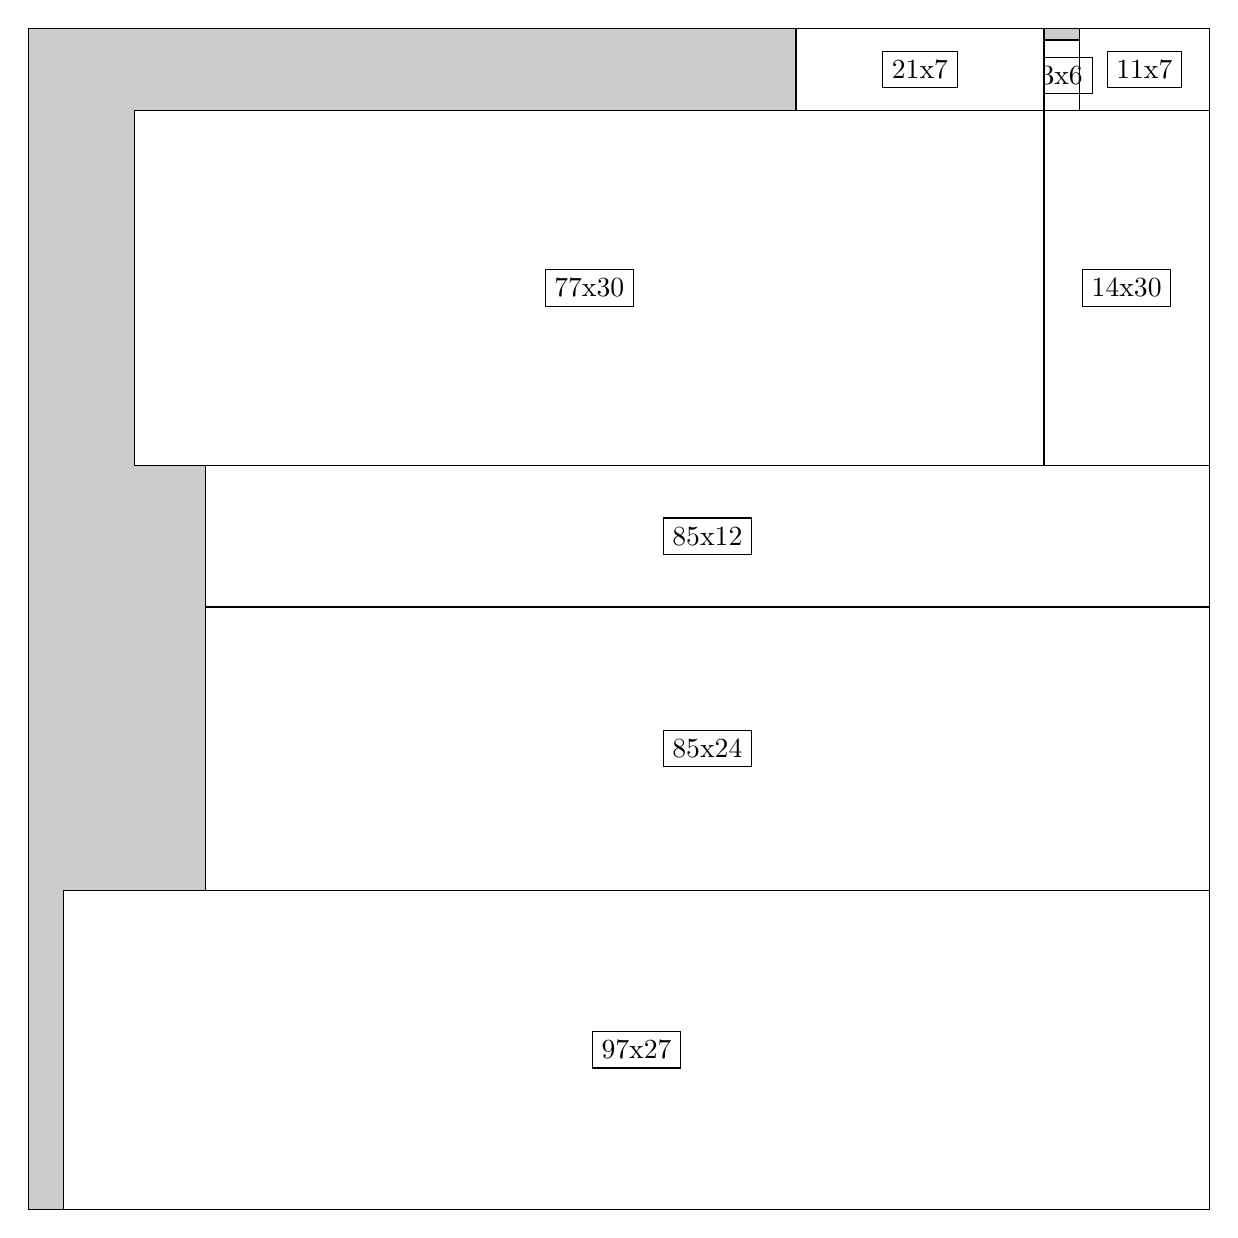
\begin{tikzpicture}[shorten >=1pt,scale=1.0,every node/.style={scale=1.0},->]
\tikzstyle{vertex}=[circle,fill=black!25,minimum size=14pt,inner sep=0pt]
\filldraw[fill=gray!40!white, draw=black] (0,0) rectangle (15.0,15.0);
\foreach \name/\x/\y/\w/\h in {97x27/0.44999999999999996/0.0/14.549999999999999/4.05,85x24/2.25/4.05/12.75/3.5999999999999996,85x12/2.25/7.6499999999999995/12.75/1.7999999999999998,14x30/12.9/9.45/2.1/4.5,11x7/13.35/13.95/1.65/1.05,3x6/12.9/13.95/0.44999999999999996/0.8999999999999999,77x30/1.3499999999999999/9.45/11.549999999999999/4.5,21x7/9.75/13.95/3.15/1.05}
\filldraw[fill=white!40!white, draw=black] (\x,\y) rectangle node[draw] (\name) {\name} ++(\w,\h);
\end{tikzpicture}


w =97 , h =27 , x =3 , y =0 , v =2619
\par
w =85 , h =24 , x =15 , y =27 , v =2040
\par
w =85 , h =12 , x =15 , y =51 , v =1020
\par
w =14 , h =30 , x =86 , y =63 , v =420
\par
w =11 , h =7 , x =89 , y =93 , v =77
\par
w =3 , h =6 , x =86 , y =93 , v =18
\par
w =77 , h =30 , x =9 , y =63 , v =2310
\par
w =21 , h =7 , x =65 , y =93 , v =147
\par
\newpage


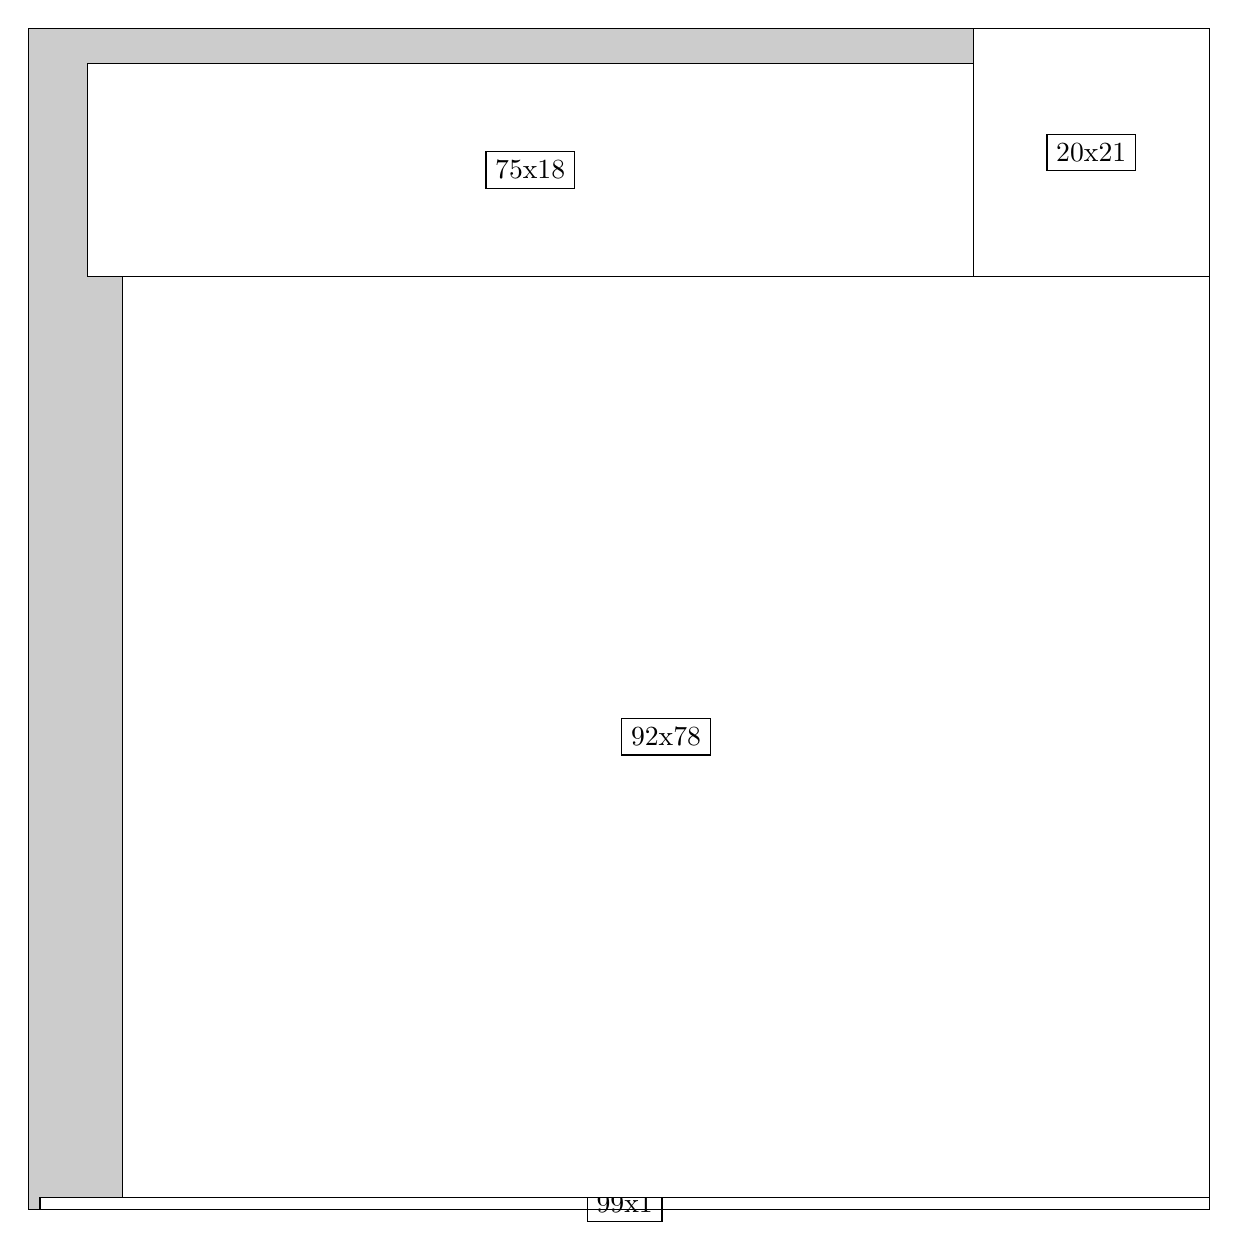
\begin{tikzpicture}[shorten >=1pt,scale=1.0,every node/.style={scale=1.0},->]
\tikzstyle{vertex}=[circle,fill=black!25,minimum size=14pt,inner sep=0pt]
\filldraw[fill=gray!40!white, draw=black] (0,0) rectangle (15.0,15.0);
\foreach \name/\x/\y/\w/\h in {99x1/0.15/0.0/14.85/0.15,92x78/1.2/0.15/13.799999999999999/11.7,20x21/12.0/11.85/3.0/3.15,75x18/0.75/11.85/11.25/2.6999999999999997}
\filldraw[fill=white!40!white, draw=black] (\x,\y) rectangle node[draw] (\name) {\name} ++(\w,\h);
\end{tikzpicture}


w =99 , h =1 , x =1 , y =0 , v =99
\par
w =92 , h =78 , x =8 , y =1 , v =7176
\par
w =20 , h =21 , x =80 , y =79 , v =420
\par
w =75 , h =18 , x =5 , y =79 , v =1350
\par
\newpage


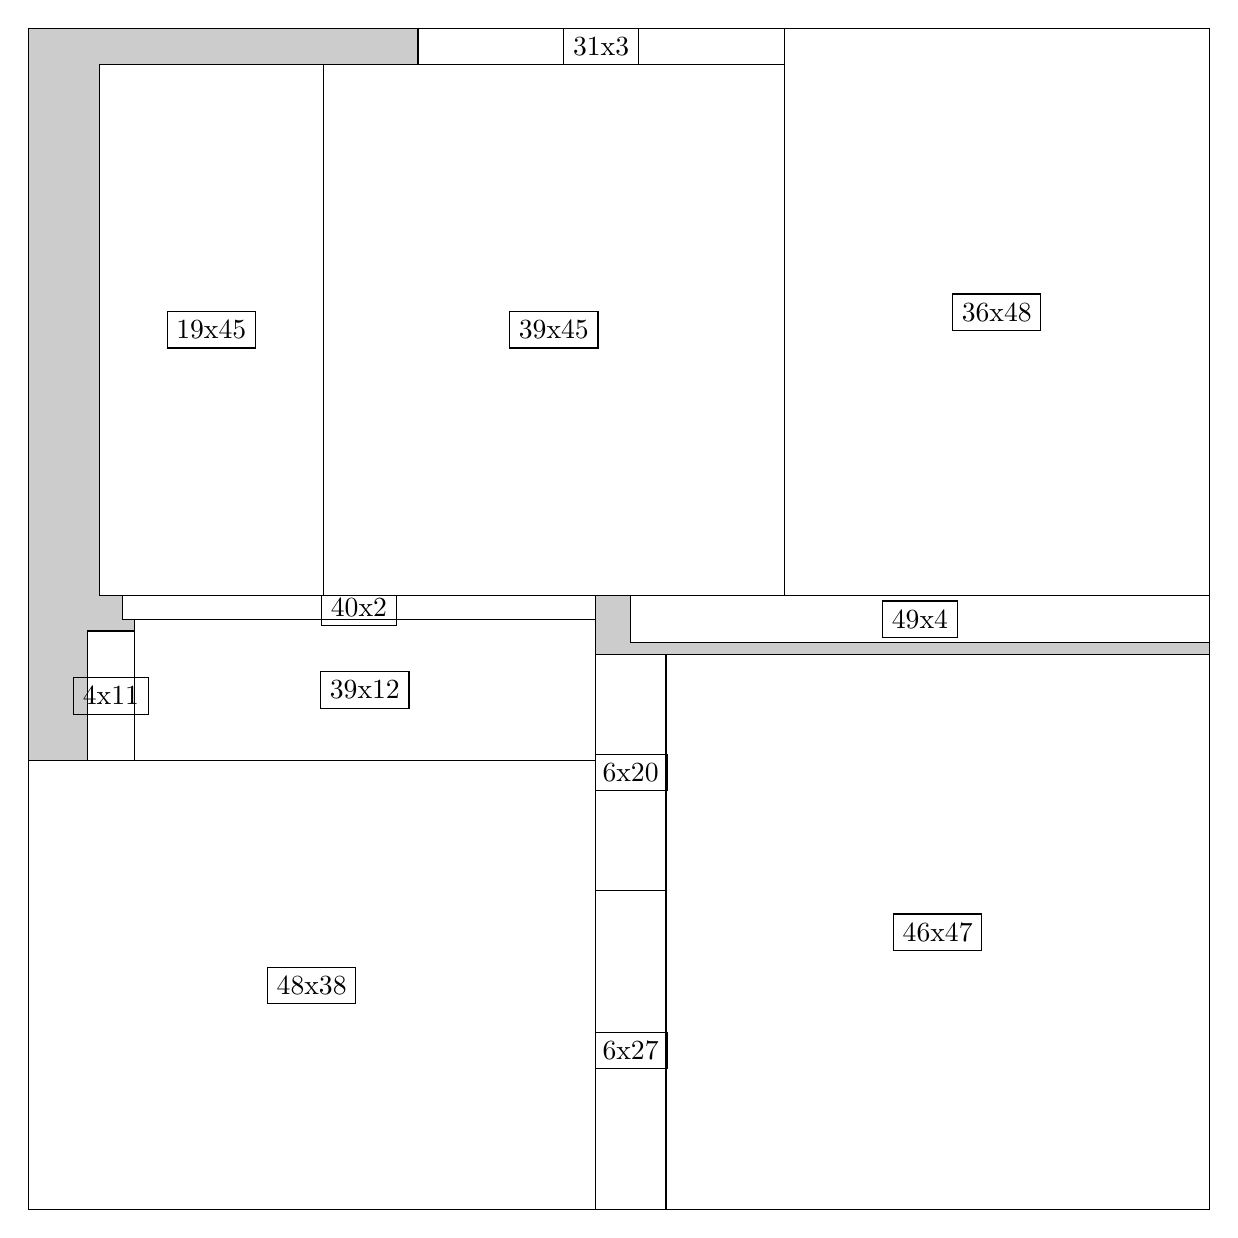
\begin{tikzpicture}[shorten >=1pt,scale=1.0,every node/.style={scale=1.0},->]
\tikzstyle{vertex}=[circle,fill=black!25,minimum size=14pt,inner sep=0pt]
\filldraw[fill=gray!40!white, draw=black] (0,0) rectangle (15.0,15.0);
\foreach \name/\x/\y/\w/\h in {46x47/8.1/0.0/6.8999999999999995/7.05,6x27/7.199999999999999/0.0/0.8999999999999999/4.05,6x20/7.199999999999999/4.05/0.8999999999999999/3.0,49x4/7.6499999999999995/7.199999999999999/7.35/0.6,48x38/0.0/0.0/7.199999999999999/5.7,39x12/1.3499999999999999/5.7/5.85/1.7999999999999998,4x11/0.75/5.7/0.6/1.65,40x2/1.2/7.5/6.0/0.3,36x48/9.6/7.8/5.3999999999999995/7.199999999999999,39x45/3.75/7.8/5.85/6.75,31x3/4.95/14.549999999999999/4.6499999999999995/0.44999999999999996,19x45/0.8999999999999999/7.8/2.85/6.75}
\filldraw[fill=white!40!white, draw=black] (\x,\y) rectangle node[draw] (\name) {\name} ++(\w,\h);
\end{tikzpicture}


w =46 , h =47 , x =54 , y =0 , v =2162
\par
w =6 , h =27 , x =48 , y =0 , v =162
\par
w =6 , h =20 , x =48 , y =27 , v =120
\par
w =49 , h =4 , x =51 , y =48 , v =196
\par
w =48 , h =38 , x =0 , y =0 , v =1824
\par
w =39 , h =12 , x =9 , y =38 , v =468
\par
w =4 , h =11 , x =5 , y =38 , v =44
\par
w =40 , h =2 , x =8 , y =50 , v =80
\par
w =36 , h =48 , x =64 , y =52 , v =1728
\par
w =39 , h =45 , x =25 , y =52 , v =1755
\par
w =31 , h =3 , x =33 , y =97 , v =93
\par
w =19 , h =45 , x =6 , y =52 , v =855
\par
\newpage


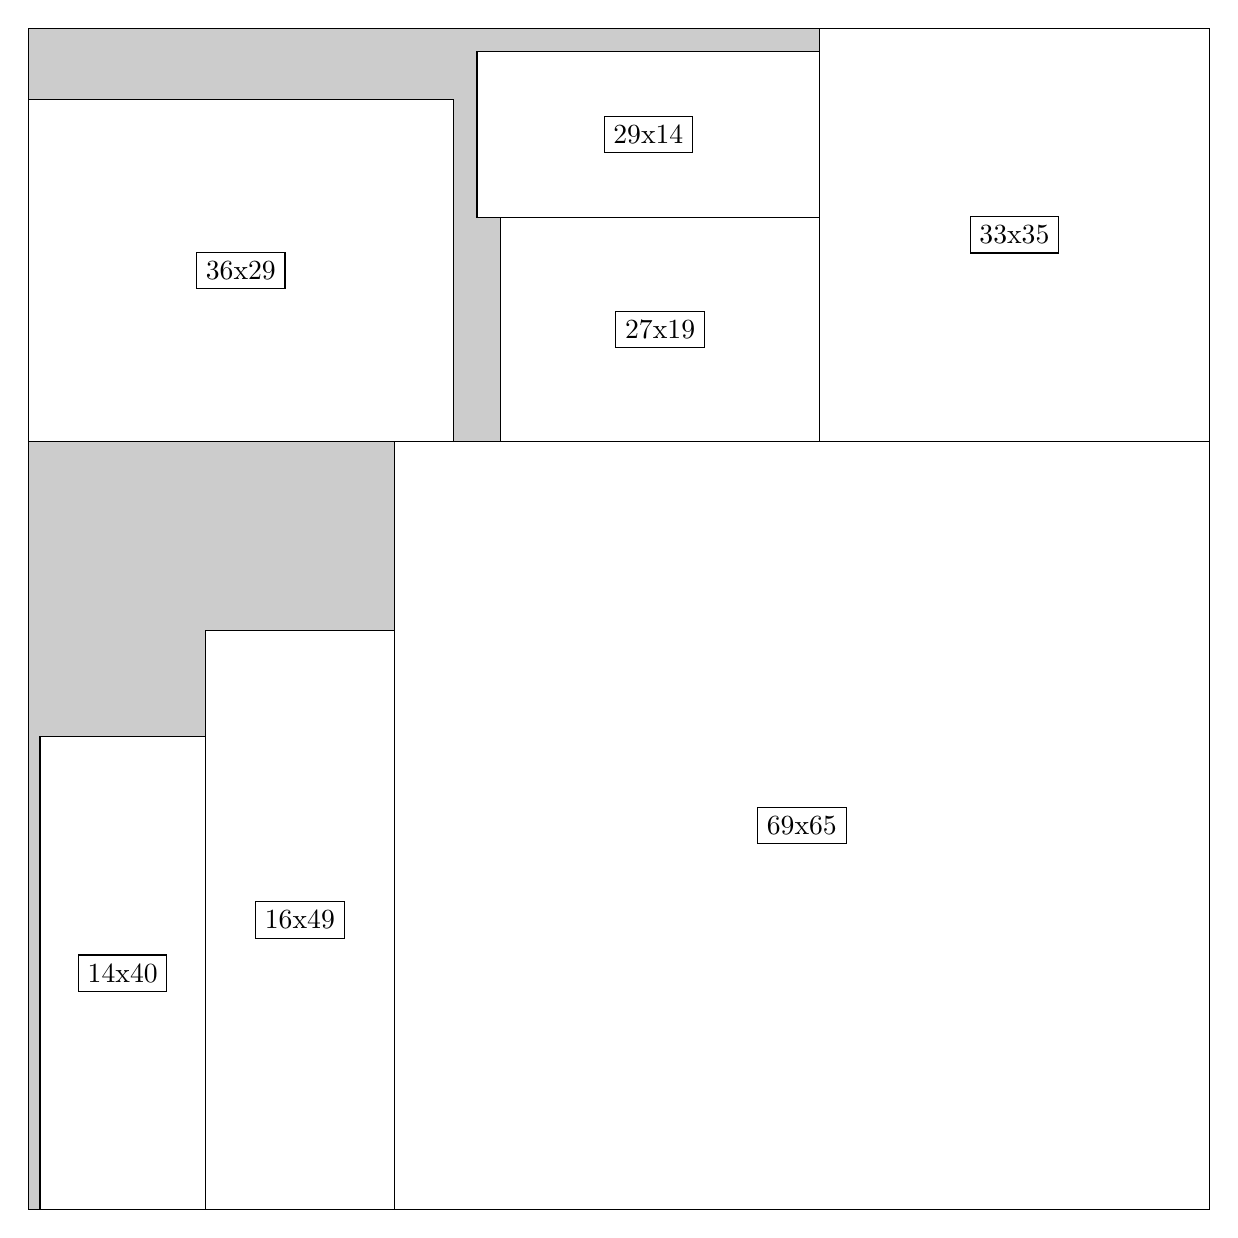
\begin{tikzpicture}[shorten >=1pt,scale=1.0,every node/.style={scale=1.0},->]
\tikzstyle{vertex}=[circle,fill=black!25,minimum size=14pt,inner sep=0pt]
\filldraw[fill=gray!40!white, draw=black] (0,0) rectangle (15.0,15.0);
\foreach \name/\x/\y/\w/\h in {69x65/4.6499999999999995/0.0/10.35/9.75,16x49/2.25/0.0/2.4/7.35,14x40/0.15/0.0/2.1/6.0,33x35/10.049999999999999/9.75/4.95/5.25,27x19/6.0/9.75/4.05/2.85,29x14/5.7/12.6/4.35/2.1,36x29/0.0/9.75/5.3999999999999995/4.35}
\filldraw[fill=white!40!white, draw=black] (\x,\y) rectangle node[draw] (\name) {\name} ++(\w,\h);
\end{tikzpicture}


w =69 , h =65 , x =31 , y =0 , v =4485
\par
w =16 , h =49 , x =15 , y =0 , v =784
\par
w =14 , h =40 , x =1 , y =0 , v =560
\par
w =33 , h =35 , x =67 , y =65 , v =1155
\par
w =27 , h =19 , x =40 , y =65 , v =513
\par
w =29 , h =14 , x =38 , y =84 , v =406
\par
w =36 , h =29 , x =0 , y =65 , v =1044
\par
\newpage


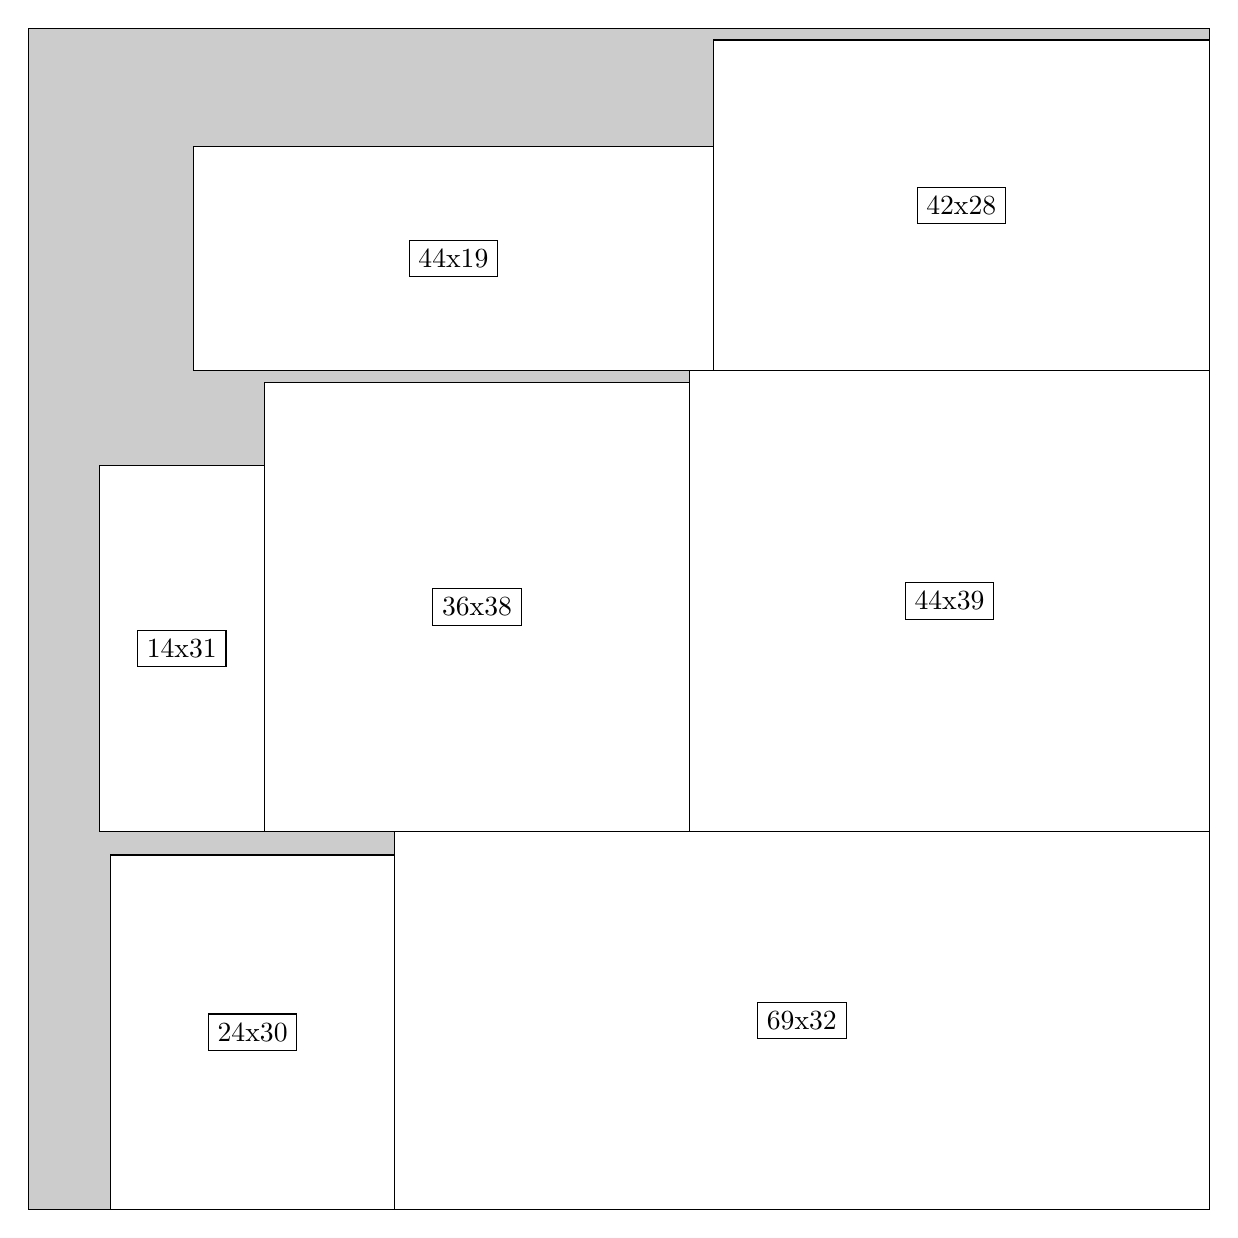
\begin{tikzpicture}[shorten >=1pt,scale=1.0,every node/.style={scale=1.0},->]
\tikzstyle{vertex}=[circle,fill=black!25,minimum size=14pt,inner sep=0pt]
\filldraw[fill=gray!40!white, draw=black] (0,0) rectangle (15.0,15.0);
\foreach \name/\x/\y/\w/\h in {69x32/4.6499999999999995/0.0/10.35/4.8,24x30/1.05/0.0/3.5999999999999996/4.5,44x39/8.4/4.8/6.6/5.85,36x38/3.0/4.8/5.3999999999999995/5.7,14x31/0.8999999999999999/4.8/2.1/4.6499999999999995,42x28/8.7/10.65/6.3/4.2,44x19/2.1/10.65/6.6/2.85}
\filldraw[fill=white!40!white, draw=black] (\x,\y) rectangle node[draw] (\name) {\name} ++(\w,\h);
\end{tikzpicture}


w =69 , h =32 , x =31 , y =0 , v =2208
\par
w =24 , h =30 , x =7 , y =0 , v =720
\par
w =44 , h =39 , x =56 , y =32 , v =1716
\par
w =36 , h =38 , x =20 , y =32 , v =1368
\par
w =14 , h =31 , x =6 , y =32 , v =434
\par
w =42 , h =28 , x =58 , y =71 , v =1176
\par
w =44 , h =19 , x =14 , y =71 , v =836
\par
\newpage


\end{document}